%% LyX 2.1.4 created this file.  For more info, see http://www.lyx.org/.
%% Do not edit unless you really know what you are doing.
\documentclass[american,fontsize=11pt,paper=a4,twoside,openright,titlepage,numbers=noenddot,headinclude,BCOR=5mm,footinclude=true,cleardoublepage=empty]{scrreprt}
\usepackage[T1]{fontenc}
\usepackage[utf8]{inputenc}
\setcounter{secnumdepth}{2}
\usepackage{color}
\usepackage{array}
\usepackage{verbatim}
\usepackage{booktabs}
\usepackage{amsmath}
\usepackage{amssymb}
\usepackage{graphicx}

\makeatletter

%%%%%%%%%%%%%%%%%%%%%%%%%%%%%% LyX specific LaTeX commands.
%% Because html converters don't know tabularnewline
\providecommand{\tabularnewline}{\\}

%%%%%%%%%%%%%%%%%%%%%%%%%%%%%% Textclass specific LaTeX commands.
% Classic Thesis Style loader
\makeatother
\input{classicthesis-config.tex}
\makeatletter

% \input@path is a list of paths where LaTeX should look for files
% LyX defines it as a single element list with the path of the main document in it
% Comes in two forms: {\string "/home/user/dir ectory/\string "/} or {/home/user/directory//}
% This is a hack to extract the bare path from the above strings
\ifcsname input@path\endcsname 
  \edef\@basepath{\expandafter\@firstofone\input@path} %remove braces
  \def\rm@quotes#1"#2"#3\@nul{\ifx\relax#2\relax #1\else #2\fi}
  \edef\@basepath{\expandafter\rm@quotes\@basepath""\@nul} %remove quotes
\else\edef\@basepath{./}\fi


\let\orig@addbibresource\addbibresource
\renewrobustcmd*{\addbibresource}[2][type=file]{\orig@addbibresource[#1]{\@basepath#2}}

% use Latin Modern instead of Computer Modern sans serif
\renewcommand{\sfdefault}{lmss}

%%%%%%%%%%%%%%%%%%%%%%%%%%%%%% User specified LaTeX commands.
\addbibresource{Bibliography.bib}
\addbibresource[label=ownpubs]{AMiede_Publications.bib}

\ExecuteBibliographyOptions{backref=true,isbn=false}

\makeatother

\usepackage{babel}
\begin{document}
\frenchspacing
\raggedbottom
\pagenumbering{roman}
\pagestyle{plain}

\begin{titlepage}
\begin{addmargin}[-10mm]{-30mm}  %%%%% symmetrical margins
\large
\hfill

\vfill{}

\begin{center}
\begingroup\color{blood} \huge \spacedallcaps{\MyTitle} \endgroup\\
\bigskip{}
\begingroup\color{blood} \Large \spacedallcaps{\mytitle} \endgroup\\
\par\end{center}

\begin{center}
\medskip{}
\spacedlowsmallcaps{\myName}
\par\end{center}

\begin{center}
\medskip{}
\par\end{center}

\begin{center}
Under the direction of
\par\end{center}

\begin{center}
\spacedlowsmallcaps{\myProf} \& \spacedlowsmallcaps{\myOtherProf}
\par\end{center}

\begin{center}
\vfill{}
\par\end{center}

\begin{center}
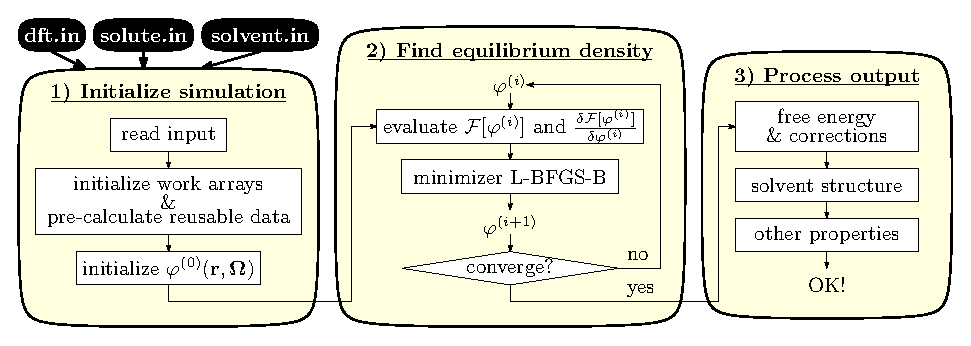
\includegraphics[width=0.5\paperwidth]{Front_Staff/mdft}\\
 \medskip{}
\par\end{center}

\begin{center}
\spacedlowsmallcaps{\mySubtitle}
\par\end{center}

\begin{center}
\spacedlowsmallcaps{\mysubtitle}
\par\end{center}

\vfill{}

\begin{center}
\bigskip{}
\par\end{center}

\begin{center}
\myTime @ \myLocation
\par\end{center}

\end{addmargin} 
\end{titlepage} 


\include{Front_Staff/Titleback}

\cleardoublepage{}

\pdfbookmark[1]{Acknowledgments}{acknowledgments}

\begin{flushright}
\textsl{When you are studying any matter, or considering any philosophy,
ask yourself only, what are the facts and what is the truth that the
facts bear out.}\\
\textsl{ Never let yourself be diverted either by what you wish to
believe, or by what you think would have beneficent social effects
if it were believed.}\\
\textsl{ But look only, and solely, at what are the facts.}
\par\end{flushright}

\begin{flushright}
--- Bertrand Russell 
\par\end{flushright}

\bigskip{}


\begingroup
\let\clearpage\relax
\let\cleardoublepage\relax 


\chapter*{Acknowledgements}

First of all, I would like to express my most respectful gratitude
to my thesis advisors, Daniel Borgis and Luc Belloni, who have developed
the main theories used in this thesis and and whose great knowledge
of liquid theory as well as the genius way of thinking and explaining
have given me a solid guide for doing this research. I would also
like to thank them for their tireless work in correcting this manuscript.

I'm grateful to Maximilien Levesque, the other main developer of MDFT
who joined the supervision of my thesis. Thanks for sharing some results
and data that have proven useful to my research.

I wish to acknowledge all the great minds willing to evaluate and
give ideas about my work: \textcolor{red}{(noms des jurés)}, thank
you for agreeing to be part of the jury of this thesis.

As a master student issue from pure chemistry speciality, a lack of
knowledge about Informatics brought to me a lot of difficulties. I
would like to express my sincere gratitude to my colleagues Pierre
Kestener, Matthieu Haefele, and Yacine Ould-Rouis for their huge aid
in Informatics and very useful advices during this thesis.

This thesis was produced at\textit{ Maison de la Simulation, CEA Saclay},
financially supported by the scholarship \textcolor{red}{IDEX-CEA}.
I acknowledge all the organizations and staff that gave me the chance
to have this three-year experience.

I am also grateful to Thomas Wiggins for help in correcting the huge
amount of grammar faults in this manuscript.

I'm deeply indebted to my tutors during my bachelor and master, respectively
Mr. Hongwei Tan and Mrs. Michelle Gupta, whose clear logic and warm
encouragement gave me all that I needed to be in love with theoretical
chemistry.

Finally I would like to thank my father, who made the right decision
to send me here in France and support me in every aspect.

\endgroup


\cleardoublepage{}

\pagestyle{scrheadings}

%*************************
% Table of Contents
%*************************
%\phantomsection
\refstepcounter{dummy}
\pdfbookmark[1]{\contentsname}{tableofcontents} 
\setcounter{tocdepth}{2} % <-- 2 includes up to subsections in the ToC 
\setcounter{secnumdepth}{3} % <-- 3 section numbers up to subsubsections 
\manualmark 
\markboth{\spacedlowsmallcaps{\contentsname}}{\spacedlowsmallcaps{\contentsname}} 
\tableofcontents  
\automark[section]{chapter} 
\renewcommand{\chaptermark}[1]{\markboth{\spacedlowsmallcaps{#1}}{\spacedlowsmallcaps{#1}}} \renewcommand{\sectionmark}[1]{\markright{\thesection\enspace\spacedlowsmallcaps{#1}}} 

\clearpage{}

\begingroup
\let\clearpage\relax
\let\cleardoublepage\relax

%*************************
% List of Figures     
%*************************
%\phantomsection
\refstepcounter{dummy}
%\addcontentsline{toc}{chapter}{\listfigurename}
\pdfbookmark[1]{\listfigurename}{lof}
\listoffigures

\vspace{4ex}

%*************************
% List of Tables
%*************************
%\phantomsection
\refstepcounter{dummy}
%\addcontentsline{toc}{chapter}{\listtablename}
\pdfbookmark[1]{\listtablename}{lot}
\listoftables

\vspace{4ex}

%*************************
% Notations
%*************************
%\phantomsection
\refstepcounter{dummy}
\pdfbookmark[1]{Notations}{notations}
\markboth{\spacedlowsmallcaps{Notations}}{\spacedlowsmallcaps{Notations}}
\chapter*{Notations} 

\hspace{-0.5em}%
\begin{tabular}{>{\raggedright}p{3.3em}l}
$\varOmega$ & Grand potential {[}$\mathrm{kJ\cdot mol^{-1}}${]}\tabularnewline
\end{tabular}

\hspace{-1.5em}%
\begin{tabular}{>{\raggedright}p{3.3em}l}
$\varXi$ & Grand partition function, dimensionless\tabularnewline
\end{tabular}

\hspace{-1.5em}%
\begin{tabular}{>{\raggedright}p{3.3em}l}
$F$ & Helmholtz free energy {[}$\mathrm{kJ\cdot mol^{-1}}${]}\tabularnewline
\end{tabular}

\hspace{-1.5em}%
\begin{tabular}{>{\raggedright}p{3.3em}l}
$\mathcal{F}[\rho]$ & Solvation free energy functional {[}$\mathrm{kJ\cdot mol^{-1}}${]}\tabularnewline
\end{tabular}

\hspace{-1.5em}%
\begin{tabular}{>{\raggedright}p{3.3em}l}
$\rho(\mathbf{r},\mathbf{\Omega})$ & Density variable of solvent {[}$\textrm{\AA}^{-3}${]}\tabularnewline
\end{tabular}

\hspace{-1.5em}%
\begin{tabular}{>{\raggedright}p{3.3em}l}
$\mathbf{\Omega}$ & Orientation variable in laboratory coordinate system, $\mathbf{\Omega}\equiv\left(\Theta,\Phi,\Psi\right)$\tabularnewline
\end{tabular}

\hspace{-1.5em}%
\begin{tabular}{>{\raggedright}p{3.3em}l}
$\boldsymbol{\omega}$ & Orientation variable in intermolecular coordinate system, $\boldsymbol{\omega}\equiv\left(\theta,\phi,\psi\right)$\tabularnewline
\end{tabular}

\hspace{-1.5em}%
\begin{tabular}{>{\raggedright}p{3.3em}l}
$n(\mathbf{r})$ & Number density of solvent {[}$\textrm{\AA}^{-3}${]}, $n(\mathbf{r})=\int\mathrm{d}\mathbf{\Omega}\rho(\mathbf{r},\mathbf{\Omega})$\tabularnewline
\end{tabular}

\hspace{-1.5em}%
\begin{tabular}{>{\raggedright}p{3.3em}>{\raggedright}p{0.87\columnwidth}}
$\rho_{0}$ & Bulk solvent angular density, $n_{0}=\left(\int\mathrm{d}\mathbf{\Omega}\right)\rho_{\text{0}}$
is the bulk solvent number density, both of unity {[}$\mathrm{\textrm{\AA}^{-3}}${]};
in this thesis, $n_{0}=0.0332891$ is used as given by the original
code\tabularnewline
\end{tabular}

\hspace{-1.5em}%
\begin{tabular}{>{\raggedright}p{3.3em}l}
$\mathcal{F}_{\mathrm{id}}[\rho]$ & Ideal free energy functional {[}$\mathrm{kJ\cdot mol^{-1}}${]} \tabularnewline
\end{tabular}

\hspace{-1.5em}%
\begin{tabular}{>{\raggedright}p{3.3em}l}
$\mathcal{F}_{\mathrm{ext}}[\rho]$ & External free energy functional {[}$\mathrm{kJ\cdot mol^{-1}}${]} \tabularnewline
\end{tabular}

\hspace{-1.5em}%
\begin{tabular}{>{\raggedright}p{3.3em}l}
$V_{\mathrm{ext}}$ & External potential imposed by the solute {[}$\mathrm{kJ\cdot mol^{-1}}${]} \tabularnewline
\end{tabular}

\hspace{-1.5em}%
\begin{tabular}{>{\raggedright}p{3.3em}l}
$\mu$ & Chemical potential of unity {[}$\mathrm{kJ\cdot mol^{-1}}${]}\tabularnewline
\end{tabular}

\hspace{-1.5em}%
\begin{tabular}{>{\raggedright}p{3.3em}l}
$\mathcal{F}_{\mathrm{exc}}[\rho]$ & Excess free energy functional {[}$\mathrm{kJ\cdot mol^{-1}}${]}\tabularnewline
\end{tabular}

\hspace{-1.5em}%
\begin{tabular}{>{\raggedright}p{3.3em}l}
$\gamma$ & Normalized gradient of excess free energy functional, dimensionless\tabularnewline
\end{tabular}

\hspace{-1.5em}%
\begin{tabular}{>{\raggedright}p{3.3em}l}
$g$ & Pair distribution function (PDF), dimensionless\tabularnewline
\end{tabular}

\hspace{-1.5em}%
\begin{tabular}{>{\raggedright}p{3.3em}>{\raggedright}p{0.87\columnwidth}}
$h$ & Pair correlation function (PCF), or total correlation function (TCF)
in certain references, dimensionless\tabularnewline
\end{tabular}

\hspace{-1.5em}%
\begin{tabular}{>{\raggedright}p{3.3em}l}
$c$ & Direct correlation function (DCF), dimensionless\tabularnewline
\end{tabular}

\hspace{-1.5em}%
\begin{tabular}{>{\raggedright}p{3.3em}l}
$R_{\mu'\mu}^{m}$ & Generalized spherical harmonics (GSH)\tabularnewline
\end{tabular}

\hspace{-1.5em}%
\begin{tabular}{>{\raggedright}p{3.3em}l}
$\Phi_{\mu u}^{mnl}$ & Rotational invariant bases defined in appendix \ref{chpt:rotational-invariant-expansion}\tabularnewline
\end{tabular}

\hspace{-1.5em}%
\begin{tabular}{>{\raggedright}p{3.3em}l}
$\mathbf{P}$ & Polarization {[}$\mathrm{\textrm{\AA}^{-3}}${]}\tabularnewline
\end{tabular}

\hspace{-1.5em}%
\begin{tabular}{>{\raggedright}p{3.3em}l}
$q_{e}$ & Elementary charge, $q_{e}=1.602176565\cdot10^{-19}\,\mathrm{[C]}$\tabularnewline
\end{tabular}

\hspace{-1.5em}%
\begin{tabular}{>{\raggedright}p{3.3em}l}
$q$ & Charge of unity $\mathrm{[C]}$; $\mathfrak{q}=q/q_{e}$ is the number
charge, dimensionless\tabularnewline
\end{tabular}

\hspace{-1.5em}%
\begin{tabular}{>{\raggedright}p{3.3em}l}
$\varepsilon_{0}$ & Vacuum permittivity, $\varepsilon_{0}=8.854187817\cdot10^{-12}\,\mathrm{[C^{2}\cdot J^{-1}\cdot m^{-1}]}$\tabularnewline
\end{tabular}

\hspace{-1.5em}%
\begin{tabular}{>{\raggedright}p{3.3em}l}
$\varepsilon$ & Dielectric constant (relative permittivity) of solvent, dimensionless\tabularnewline
\end{tabular}

\hspace{-1.5em}%
\begin{tabular}{>{\raggedright}p{3.3em}l}
$N_{\mathrm{A}}$ & Avogadro constant, $N_{\mathrm{A}}=6.02214129\cdot10^{23}\,\mathrm{[mol^{-1}]}$\tabularnewline
\end{tabular}

\hspace{-1.5em}%
\begin{tabular}{>{\raggedright}p{3.3em}>{\raggedright}p{0.87\columnwidth}}
$f_{Q}$ & $f_{Q}=q_{e}^{2}10^{-3}N_{\mathrm{A}}/(4\pi\varepsilon_{0}10^{-10})$,
electrostatic potential unit so that $f_{Q}\cdot\mathfrak{q}^{2}/r$
is in {[}$\mathrm{kJ\cdot mol^{-1}}${]}, where $\mathfrak{q}$ is
the number charge without unity, $r$ in {[}$\textrm{\AA}${]}\tabularnewline
\end{tabular}

\hspace{-1.5em}%
\begin{tabular}{>{\raggedright}p{3.3em}l}
$K_{\mathrm{B}}$ & Boltzmann constant, $K_{\mathrm{B}}=1.3806488\cdot10^{-23}\,[\mathrm{J\cdot K^{-1}}]$\tabularnewline
\end{tabular}

\hspace{-1.5em}%
\begin{tabular}{>{\raggedright}p{3.3em}l}
$\beta$ & $\beta=\left(K_{\mathrm{B}}T\right)^{-1}$, reciprocal of the thermodynamic
temperature {[}$\mathrm{mol\cdot kJ^{-1}}${]}\tabularnewline
\end{tabular}

\vspace{4ex}

%*************************
% Acronyms
%*************************
%\phantomsection
\refstepcounter{dummy}
\pdfbookmark[1]{Acronyms}{acronyms}
\markboth{\spacedlowsmallcaps{Acronyms}}{\spacedlowsmallcaps{Acronyms}}
\chapter*{Acronyms}
\begin{acronym}[UML]
  \acro{DCF}{direct correlation function}
  \acro{DFT}{discret Fourier transform, also refers to density functional theory}
  \acro{FE}{function evaluation}
  \acro{FFT}{fast Fourier transform}
  \acro{FGSHT}{fast generalized spherical harmonic transform}
  \acro{GSH}{generalized spherical harmonic}
  \acro{GSHT}{generalized spherical harmonic transform}
  \acro{HNC}{hypernetted-chain (approximation)}
  \acro{HRF}{homogeneous reference fluid (approximation)}
  \acro{IET}{integral equation theory}
  \acro{MC}{Monte Carlo}
  \acro{MD}{molecular dynamics}
  \acro{MDFT}{molecular density functional theory}
  \acro{MOZ}{molecular Ornstein-Zernike (equation)}
  \acro{MRSO}{molecule rotation symmetry order, $s=1$ or 2 according to symmetry axis}
  \acro{OZ}{Ornstein-Zernike (equation)}
  \acro{PCF}{pair correlation function}
  \acro{PDF}{pair distribution function}
  \acro{QM}{quantum mechanics} 
  \acro{RDF}{radial distribution function}
  \acro{RPF}{radial polarization function}
\end{acronym}              

\endgroup

\cleardoublepage{}


\cleardoublepage{}

\pagenumbering{arabic}


\chapter{Introduction\label{chpt:introduction}}

This thesis is about to develop an original numerical toolkit for
physical chemists and structural biologists, based on the molecular
density functional theory (\acs{MDFT}), which makes it possible to
predict efficiently, and with a microscopic accuracy, the solvation
properties of arbitrary molecular objects in arbitrary molecular solvents
(mainly water). This introduction will help to understand the objective
of this thesis, it explains why people are interested in the nature
of solvation, and where we are in the computing trends in solvation
simulation.


\section{Simulation of solvent effects}

Solvation is a fundamental phenomenon in chemistry. The chemical behavior
of lots of systems has a strong dependence on the nature of solvent.
For example, for some popular issue as metal-organic reacting center
\citep{Mn-oxo,PCET}, or pharmaceutical etudes \citep{drug_1_Perlovich,drug_2_Perlovich,drug_3}.
The solvation properties required by etudes are very variable, such
as the Gibbs free energy of solvation, solubility, partition coefficient,
saturated vapor pressure, pH value, as well as the 3D solvation structure,
etc. Overall, the interest of these solvation properties comes from
many domains, such as chemistry, biochemistry, pharmaceutics, medicine,
environmental and agrochemical industries. Unlike the well-studied
quantum mechanics (\acs{QM}) for chemical interaction and macroscopic
finite element model for physical process, the theories of solvation
are very variable and still under developing, owing to the ambiguous
compromise between the accuracy and the computing cost. In a word,
the studies in this domain are quite important and vibrant.

\begin{figure}[h]
\centering{}\textcolor{red}{}%
\begin{minipage}[t]{1\textwidth}%
\begin{center}
\includegraphics[width=1\columnwidth]{_figure/solvation}\caption[The solvation process]{The solvation process.\label{fig:Process-of-solvation} To a thermodynamic
system, whose properties only depends on the initial and final states,
it can go through different paths. The physical process of solvation
(left path)takes the solute from vacuum into bulk solvent, progressively
passing through the vacuum-liquid interface. Theoretically, the solvation
energy is defined as the energy consumed in such a progress. In theoretical
studies, the process can be decomposed to some artificial unphysical
process (right path), involving the growth of an uncharged solute-sized
cavity within the bulk solvent, the transfer of the solute charge
distribution from vacuum into the cavity, and the interaction between
the solute and solvent, etc.}

\par\end{center}%
\end{minipage}
\end{figure}


To change a phenomenon to a model, we must understand its process.
Solvation is defined as the process of moving a molecule from the
gas phase (or vacuum) to a condensed phase (figure \ref{fig:Process-of-solvation}),
which builds a stabilizing interaction with the solute (or solute
moiety like protein residues, interfaces, etc.) \citep{iupac}. Such
interactions are mostly classical, involving electrostatic forces
and van der Waals forces, with also chemically more specific effects
such as hydrogen bond formation, and quantic effects for some small
solvents whose vibrational or rotational energy states is at the same
magnitude as $k_{\mathrm{B}}T$, etc. \citep{Gray-Gubbins}.

As not all kinds of interactions is important in applications, according
to the usage, different models and methods are developed.

In the most of the 20th century \citep{Cramer_1999}, the study of
solvation effects has been dominated by continuum (implicit) models,
which is simply depending on the dielectric constants and not costly
on computation resource. They provide an accurate way to treat the
strong, long-range electrostatic interactions which dominate many
solvation phenomena, but lack of detail informations in the first
solvation shell. The later, which mainly includes the cavity formation
energy and solute-solvent van der Waals interactions, is often rudely
treat by introducing an artificial form of cavity, that links to the
form of solute. And the methods for electrostatic interactions involves
like generalized Born model, or through better estimates via Poisson-Boltzmann
calculations. They are widely integrated within \acs{QM} simulations
of the solvent, by add extra solvation terms onto the Fock or Kohn-Sham
operator \citep{Jensen,scrf,Tomasi_1994_implicit_model}. However,
the improper treatment of the first-shell, where the microscopic interactions
are primarily located, often introduce sometimes huge error in free
energy evaluation, especially for polar solvents (like water), despite
the accuracy that the \acs{QM} calculation alone can achieve. Therefore,
classical molecular simulations, which describing the individual solvent
molecules (explicit), particularly the molecular dynamics (\acs{MD})
and Monte Carlo method (\acs{MC}), became the alternative solution
during the last few decades. They generate trajectories and configurations,
then estimate free energy changes by statistical mechanic technics,
such as free energy perturbation (FEP) theory or thermodynamic integration
(TI) \citep{Jorgensen_1995_MC}. These calculation is very demanding
on computing cost, due to the requirement of many (hundreds or thousands
of) solvent molecules to form a realistic model.

Recently, a third domain of theory to describe solvent, based on the
statistical mechanics of fluid, is growing rapidly. It is generally
called liquid theory, involves mainly the integral equation theory
(\acs{IET}), and the classical density functional theory for liquids.
These approaches are cope to give the molecular nature of the first-shell,
but without calculate all the instantaneous micro-states with respect
to time, which can be integrated over positions and momentums theoretically.
Therefore, they are of magnitudes faster than those simulations by
micro-states.

The integral equation theory (\acs{IET}) is about solving the Ornstein-Zernike
(\acs{OZ}) equation with a specific closure equation \citep{Hensen-McDonald,Gray-Gubbins}.
It was firstly limited to so called ``simple liquid'' - a system
of spherical particles. A part, Chandler and Andersen in 1971 \citep{Chandler_1972_RISM}
developed the reference interaction site model (\acs{RISM}), which
discretizes the distribution and correlation functions into a site-site
set of functions, and solve the \acs{OZ} equation in matrix \citep{hirata_molecular_2004}.
Another part, Blum \citep{Blum_I,Blum_II}, Fries and Patey \citep{Fries_Patey_1985}
extend the \acs{OZ} equation to molecular case, where the distribution
and correlation functions depend on both position and orientation.
In their theory, the orientation part of \acs{OZ} equation is simplified
by expending the distribution and correlation functions on Wigner
generalized spherical harmonics.

The classical density functional theory approach deal with inhomogeneous
liquids, which uses the same variation principle and minimization
strategy \citep{mermin_thermal_1965,Evans_1979,Hansen_1987} as electronic
density functional theory \acs{DFT} that treats electric interactions
and has a great success in computational chemistry. It gives the Helmholtz
free energy and the equilibrium solvent density, by minimizing the
free energy functional of the solvent density in the presence of a
given external potential. Borgis and collaborators \textcolor{red}{{[}too
many ref{]}} have recently generalized it into molecular case, named
molecular density functional theory (\acs{MDFT}), where the solvent
density depends on both position and orientation, $\rho(\mathbf{r},\mathbf{\Omega})$.
The main theoretical difficulty lies in the definition of well-funded
and reliable functionals of the excess free energy $\mathcal{F}_{\mathrm{exc}}\left[\rho\right]$,
according to the geometric complexity of the solvent molecule. Some
recent researches have shown that it is cope with linear solvents
like acetonitrile, but still have little non-satisfaction with the
most complex solvent, i. e. water. \acs{MDFT} can be proved to be
mathematically equivalent to the two-component molecular \acs{IET}.

The majority of work of all these theories have been focused on water,
since it is one of the most difficult systems to model due to its
molecular geometry, ineligible multi-body interaction, quantum effect,
hydrogen bond, etc. The importance of including instantaneous polarization
in potential functions is also an issue \citep{polarisable_1,polarisable_2}.
However, since polarizable force fields are not yet in common use,
the simulations by micro-states and the liquid theory which feed on
force field also have their own limit, compared to the continuum model
which can be polarizable. The advantages and disadvantages of each
branch of theory are listed in table \ref{tab:Theories-of-solvation}.

\begin{table}[h]
\begin{centering}
\begin{tabular}{ccccc}
\toprule 
\tableheadline{Theory} & \tableheadline{Speed} & \tableheadline{Long-Range} & \tableheadline{First-Shell} & \tableheadline{Polarizable Solvent}\tabularnewline
\midrule
Continuum model & fast & yes & no & fully\tabularnewline
Simulation by time & costly & yes & yes & partially, very costly\tabularnewline
Liquid theory & fast & yes & yes & partially\tabularnewline
\bottomrule
\end{tabular}
\par\end{centering}

\caption{Theories of solvation simulation\label{tab:Theories-of-solvation}}
\end{table}


This thesis consists in the development of the \acs{MDFT}, focusing
on the generalization and algorithmic acceleration of the excess free
energy functional $\mathcal{F}_{\mathrm{exc}}$ evaluation under homogenous
reference fluid (\acs{HRF}) approximation, which will be discussed
in detail in later chapters. 


\section{Scope of this thesis}

Chapter I reviews a selection of models and methods to the solvent
effect. It includes the mainly used continuum model, the basic of
liquid theory, as well as its two frontier research domains, \acs{IET}
and \acs{MDFT}. The code structure of \acs{MDFT}, which all the
development in this thesis is based on, is also presented. There is
also a brief introduction to \acs{MD} and \acs{MC}, as well as the
generation of direct correlation function (\acs{DCF}) used in this
thesis by such methods. 

Chapter II presents all the theory developed and newly used in this
thesis. In this thesis, two algorithms of excess energy functional
evaluation are proposed, one is extension of the previous algorithm,
other is a new algorithm, that combines the molecular \acs{OZ} equation
treatment of angular part with MDFT. The output solvation properties
is mainly the two: free energy, and solvent structure.

Chapter III takes note of all the implementation result, that divided
into two aspects, the ``accuracy'', which involves comparisons between
algorithms, and with \acs{IET} and \acs{MD} results; and the ``efficiency'',
which evaluate the computing cost of the code, both in sequential
and parallelized version.

Chapter VI gives some application to ions and molecules.



\ctparttext{\textcolor{red}{(Chapter introduction is to clear the motivation
and relation between sections.)}\\
\medskip{}
This chapter is summery of all the previous work that this thesis
is based on.\\
\medskip{}
In section \ref{chpt:models}, we begin by introducing the models
used in our study, as well as some other models in different scale
of description, to make our choice of model reasonable. \\
\medskip{}
Once the model is chosen, all the theories become mathematical problems.
Section \ref{chpt:statistical-mechanics} reviews some basic concepts
of statistical mechanics for liquid (liquid theory), which present
the deduction of formalisms from the model of the system, without
introducing any artificial term. The following two sections, section
\ref{chpt:iem} and \ref{chpt:mdft} give two frontier domains of
the liquid theory: the integral equation theory (\acs{IET}), and
the molecular density functional theory (\acs{MDFT}) that this thesis
works on. The mathematical equivalence between these two theories
is therefore clear, presented in section \ref{chpt:mdft}, which gives
us the idea to use the expansion technics in \acs{IET} to serve \acs{MDFT}.\\
\medskip{}
After all, a brief introduction of the simulations depending on micro
configuration, here referring to molecular dynamics (\acs{MD}) and
Monte Carlo (\acs{MC}) method, is made in section \ref{chpt:reference-method},
to the purpose to explain how the direct correlation functions (\acs{DCF})
used by this thesis are obtained.}


\part{State of the Art: Solvation, Models and Methods}

\cleardoublepage{}

\appendix

\part{Appendix}


\chapter{Basics of Algorithm Complexity\label{chpt:computing-performance}}

Algorithm complexity is one of crucial criteria to evaluate the theoretical
performance of the code, as defined below:

Let $f$ and $g$ be two real (or even complex) functions defined
over the natural numbers $\mathbb{N}$. We write
\begin{equation}
f=O(g)
\end{equation}
if there is a constant $c>0$ such that from a certain number $n>n_{0}$
we always have $\left|f(n)\right|\leq c\left|g(n)\right|$. The $O$
is also named as the big-O notation \citep{Complexity}, or order
of growth. Figure \ref{fig:order-of-growth} shows the growth tendency
of some frequent functions; from this we can conclude the following:
\begin{equation}
O(1)>O(\log_{2}n)>O(n)>O(n\log_{2}n)>O(n^{2})>O(2^{n})>O(n!)
\end{equation}

\begin{figure}[h]
\begin{centering}
\includegraphics[width=0.75\textwidth]{_figure/orders-of-growth}
\par\end{centering}
\caption{Function growth\label{fig:order-of-growth}}
\end{figure}

In this thesis, the big-O notation is used to measure algorithm complexity.
Other notations can also be used for the same purpose, such as:
\begin{itemize}
\item $f=o(g)$ if $f(n)/g(n)\rightarrow0$, $n\rightarrow\infty$
\item The inverse of big-O notation $f=\Omega(g)$ if $g=O(f)$
\item The notation $f=\Theta(g)$ means that both $f=O(g)$ and $g=O(f)$
hold, and we can also say they are of the same order.
\end{itemize}
In developing code we always search for algorithms with a lower algorithm
complexity. Ideally, the implementation of code matches the model
and has the same growth tendency as its complexity. But in the practical
case, overheads and memory delay can also limit the performance.


\cleardoublepage{}

%*************************
% Bibliography 
%*************************
% work-around to have small caps also here in the headline
\manualmark \markboth{\spacedlowsmallcaps{\bibname}}{\spacedlowsmallcaps{\bibname}}
%\phantomsection
\refstepcounter{dummy}
\addtocontents{toc}{\protect\vspace{\beforebibskip}}
% to have the bib a bit away from the rest in the toc
\addcontentsline{toc}{chapter}{\tocEntry{\bibname}}

\label{app:bibliography}

\printbibliography

\end{document}
